\documentclass[a4paper, 12pt]{article}
\usepackage[utf8]{inputenc}
\usepackage[T1]{fontenc}
\usepackage{graphicx}
\usepackage{lipsum}
\usepackage{geometry}
\usepackage{titlesec}
\usepackage{times}
\usepackage{hyperref}
\usepackage{amsmath}
\usepackage[linesnumbered,ruled,vlined]{algorithm2e}
\usepackage{listings}
\usepackage{color}
\usepackage{fancyhdr}
\geometry{a4paper, margin=0.75in}
%\geometry{left=2.5cm, right=2.5cm, top=2.5cm, bottom=2.5cm}
\pagestyle{fancy}
\fancyhf{} % Clear all header and footer fields
\fancyhead[L]{<EAMS>}
\fancyhead[C]{Detailed Project Report} % Centrally aligned header
\fancyhead[R]{<Version 1.0>}
\fancyfoot[C]{\thepage} % Centrally aligned footer with page number
\definecolor{codegreen}{rgb}{0,0.6,0}
\definecolor{codegray}{rgb}{0.5,0.5,0.5}
\definecolor{codepurple}{rgb}{0.58,0,0.82}
\definecolor{backcolour}{rgb}{0.95,0.95,0.92}

\lstdefinestyle{mystyle}{
    backgroundcolor=\color{backcolour},
    commentstyle=\color{codegreen},
    keywordstyle=\color{magenta},
    numberstyle=\tiny\color{codegray},
    stringstyle=\color{codepurple},
    basicstyle=\ttfamily\footnotesize,
    breakatwhitespace=false,
    breaklines=true,
    captionpos=b,
    keepspaces=true,
    numbers=left,
    numbersep=5pt,
    showspaces=false,
    showstringspaces=false,
    showtabs=false,
    tabsize=2
}

\lstset{style=mystyle}
\begin{document}
\begin{titlepage}
    \centering
    \vspace{3.5cm}
    
\includegraphics[width=0.5\textwidth]{NU-logo.jpg}\par\vspace{1cm}
    
\includegraphics[width=0.5\textwidth]{FAST.png}\par\vspace{1cm}
    \vspace{2cm}
    {\scshape\Large\textbf {Detailed Project Report} \par}
    \vspace{2cm}
    {\scshape\LARGE\textbf {Employee Attendance Management System} \par}
    \vspace{0.25cm}
    {\scshape\Large Version 1.0 \par}
    \vspace{2cm}
    {\scshape\Large Instructor Ms. Fizza Mansoor (BCS-5E) \par}
    \vspace{0.25cm}
    {\scshape\Large Database Systems (CS-2005) \par}
    \vspace{2cm}
    \begin{itemize}
    \item {\scshape\Large Muhammad Hamza (K21-4579) \par}
    \vspace{0.25cm}
    \item {\scshape\Large Muhammad Salar (K21-4619) \par}
    \end{itemize}
    \vfill
    \vspace{1cm}    
    {Foundation of Advancement of Science and Technology \par}
    {National University of Computer and Emerging Sciences \par}
    {Department of Computer Science \par}
    {Karachi, Pakistan \par}
    {Thursday, December 7, 2023 \par}
\end{titlepage}

\tableofcontents
\newpage

\section*{\centering SOFTWARE REQUIREMENT SPECIFICATIONS}

\section{Introduction}
% Your introduction content here

\subsection{Purpose Of Document}
This document is a Software Requirements Specification (SRS) that provides a detailed overview of the Employee Attendance Management System project. It describes the problem that needs to be solved, the proposed solution, the scope of the project, the features and functions of the system, the data model, the tools and techniques used, the project timeline, and the conclusion. This document is intended to help the development team, the stakeholders, and any other parties involved in the project to have a clear understanding of the requirements and goals.

\subsection{Intended Audience}
The intended audience for this document includes:
\begin{itemize}
    \item \textbf{Development Team: }This group comprises the developers, coders, and software architects tasked with the creation, execution, and validation of the Employee Attendance Management System.
    \item \textbf{Project Managers: }These are the individuals charged with the administration of the project, the distribution of resources, and the assurance of its congruence with the company’s objectives and deadlines.
    \item \textbf{Stakeholders: }These are the people or entities within the company who have a significant interest in the fruitful development and implementation of the Employee Attendance Management System. This category may encompass senior leadership, supervisors, and staff members who will utilize the system.
    \item \textbf{End Users: }These are the staff members and supervisors in the company who will engage with and derive advantages from the Employee Attendance Management System upon its rollout.
\end{itemize}

\subsection{Definition of Terms, Acronyms and Abbreviations}
  \begin{tabular}{|c|c|}
    \hline
    \textbf {Term} & \textbf {Description}\\
    \hline
    ASP & Active Server Pages, a server-side script engine for dynamically generated web pages\\
    \hline
    SSL & Secure Socket Layer, a protocol for establishing encrypted links between networked computers\\
    \hline
    SQL & Structured Query Language, a standardized language for managing relational databases\\
    \hline
    JSON & JavaScript Object Notation, a data-interchange format that is easier for humans\\
    \hline
    SRS & Software Requirements Specification, a document for the software requirements for a system\\
    \hline
    SDS & Software Design Specification, a document for the design details of a system\\
    \hline
    HTML & Hyper-Text Markup Language, the standard markup language for web pages\\
    \hline
    CSS & Cascading Style Sheets, a language used for the presentation of a document in HTML or XML\\
    \hline
    TLS & Transport Layer Security, a protocol to provide communications security over a network\\
    \hline
    APIs & Application Programming Interface, a set of routines, and protocols for software applications\\
    \hline
  \end{tabular}

\subsection{Document Convention}
This document uses font size 16 for main headings, 14 for sub headings and 12 for body, also the overall font style is Times New Roman. Line spacing is single (1.0)

\newpage
\section{Overall System Description}
\subsection{Project Background}
In the ever-evolving corporate landscape, adept management of tasks is essential for a company’s prosperity. The inception of this project is rooted in the difficulties that numerous organizations encounter in effectively coordinating and monitoring employee responsibilities, which often results in unmet deadlines and diminished clarity. The demand for an integrated and intuitive system has given rise to the creation of the Employee Attendance Management System. This platform endeavours to simplify the allocation, supervision, and fulfilment of tasks, thereby cultivating an orderly and efficient workplace.

\subsection{Project Scope}
The Employee Attendance Management System project is centred on constructing an online platform that streamlines efficient attendance tracking within the company. The principal features include attendance logging, absence monitoring, deleting erroneous entries, user verification, and database management. The system aims to offer a complete solution that empowers authorized individuals to oversee attendance reliably, promoting accountability and punctual adherence to work schedules. The system will deliberately exclude any features not directly related to attendance management.

\subsection{Not in Scope}
The subsequent features are categorically excluded from the purview of this project:
\begin{itemize}
    \item Complex project management capabilities that surpass basic attendance tracking.
    \item Synchronization with third-party attendance or HR management tools.
    \item Financial operations such as payroll processing or generating invoices.
\end{itemize}

\subsection{Project Objectives}
Project Objectives The project is committed to accomplishing the following goals:
\begin{itemize}
    \item Simplify the process of recording and monitoring attendance.
    \item Improve visibility in attendance tracking within the company.
    \item Offer an intuitive Employee Attendance Management System for authorized users.
    \item Showcase effective database management for handling attendance data.
\end{itemize}

\subsection{Stakeholders}
Stakeholders The system’s stakeholders encompass:
\begin{itemize}
    \item \textbf{Managers:} Accountable for scheduling employee attendance and supervising adherence to work hours.
    \item \textbf{Employees:} Individuals who will engage with the system to check in and verify their attendance records.
    \item \textbf{Database Administrators:} Entrusted with the upkeep and administration of the core database system.
\end{itemize}

\subsection{Operating Environment}
The system is designed to function within a web-based framework. The hardware requirements are inclusive of standard computing devices that have access to the internet. It will be compatible with prevalent operating systems such as Windows or Linux. Additionally, the system is built to operate seamlessly alongside web browsers like Chromium-based browsers or Firefox.

\subsection{System Constraints}
System Constraints The system is subject to the following limitations:
\begin{itemize}
    \item \textbf{Software Constraints:} The system must be compatible with designated web browsers.
    \item \textbf{Hardware Constraints:} The system requires standard computing devices that are connected to the internet.
    \item \textbf{Legal Constraints:} The system must comply with applicable data protection and privacy regulations.
    \item \textbf{User Constraints:} Users should have a basic understanding of web interfaces and operations.
\end{itemize}

\subsection{Assumptions \& Dependencies}
The system’s operation is predicated on the following:
\begin{itemize}
    \item \textbf{Assumptions:} It is presumed that users possess an elementary proficiency with web interfaces and that the organization adheres to pertinent data protection legislation.
    \item \textbf{Dependencies:} The system’s functionality is reliant on a consistent internet connection to facilitate instantaneous updates. Moreover, the progression of the project is contingent upon the accessibility of the requisite development assets.
\end{itemize}

\newpage
\section{External Interface Requirements}
\subsection{Hardware Interfaces}
The Employee Attendance Management System is an online application that is not bound by specific hardware requirements. It is engineered to function on universally available computing devices such as desktops, laptops, and palmtops. The system’s hardware interfaces are universally applicable and encompass any device equipped with web browsing functionality and internet access.

\subsection{Software Interfaces}
The system engages with the subsequent software elements:
\begin{itemize}
    \item \textbf{MySQL Database (Version 8.2.0):} The Employee Attendance Management System utilizes MySQL for its database needs, encompassing data storage, access, and administration. The MySQL database is integrated via the XAMPP server.
    \item \textbf{Express.js (Node.js Framework):} The system’s backend infrastructure is constructed with Express, a Node.js framework, which manages API calls, user authentication, and database exchanges.
    \item \textbf{React.js (Version 18):} The system’s frontend is crafted using React, ensuring a lively and adaptable user interface for the Employee Attendance Management System.
    \item \textbf{Node.js (Version 18.16.1):} Node.js operates as the server-side JavaScript environment, executing server tasks and enabling interaction between the frontend and the database.
\end{itemize}
Data Items or Messages Exchanged:
\begin{itemize}
    \item \textbf{Between Frontend and Backend:} The system utilizes JSON data formats to convey attendance records, verify user credentials, and deliver system feedback.
    \item \textbf{Between Backend and Database:} The communication involves SQL commands and their corresponding outcomes to execute database tasks.
\end{itemize}

\subsection{Communications Interfaces}
The system adheres to established web communication standards, which include:
\begin{itemize}
    \item \textbf{HTTP/HTTPS Protocols:} Utilized for data exchange between the client-side (web browser) and the server-side (Node.js/Express backend), with HTTPS ensuring encrypted and secure data transfer.
    \item \textbf{RESTful API:} The backend offers RESTful API routes to streamline interactions between the frontend and backend, covering functionalities such as attendance management, user verification, and more.
    \item \textbf{Communication Security:} The implementation of SSL or TLS protocols will be in place to safeguard data integrity during transmission.
    \item \textbf{Data Transfer Rates:} While dependent on the user’s internet speed, the system will be optimized for swift data transfer to enhance performance.
    \item \textbf{Synchronization Mechanisms:} Asynchronous communication will be employed to enable non-disruptive interactions, ensuring a smooth user experience.
\end{itemize}

\section{Functional Requirements}
\subsection{Functional Hierarchy}
For the Employee Attendance Management System project, the restructured functional hierarchy is:
\begin{itemize}
    \item \textbf{User Authentication}
    \begin{itemize}
        \item Sign In
        \item Sign Out
    \end{itemize}
    \item \textbf{Attendance Tracking}
    \begin{itemize}
        \item Record Attendance
        \item Review Attendance
        \item Approve Absence
        \item Modify Attendance Entry
        \item Remove Attendance Entry
    \end{itemize}
    \item \textbf{Employee Directory (for managers)}
    \begin{itemize}
        \item Register Employee
        \item Browse Employee Records
        \item Update Employee Information
        \item Terminate Employee Record
    \end{itemize}
    \item \textbf{Attendance Reporting (for managers)}
    \begin{itemize}
        \item Generate Attendance Report
        \item Access Attendance History
        \item Edit Attendance Report
        \item Discard Attendance Report
    \end{itemize}
    \item \textbf{Employee Interface}
    \begin{itemize}
        \item Access Personal Profile
        \item Check Attendance Status
        \item Confirm Attendance
    \end{itemize}
\end{itemize}
This hierarchy outlines the primary operations of the Employee Attendance Management System and its organizational structure.

\subsection{Use Cases}
\subsubsection{Attendance Management System}
\begin{center}
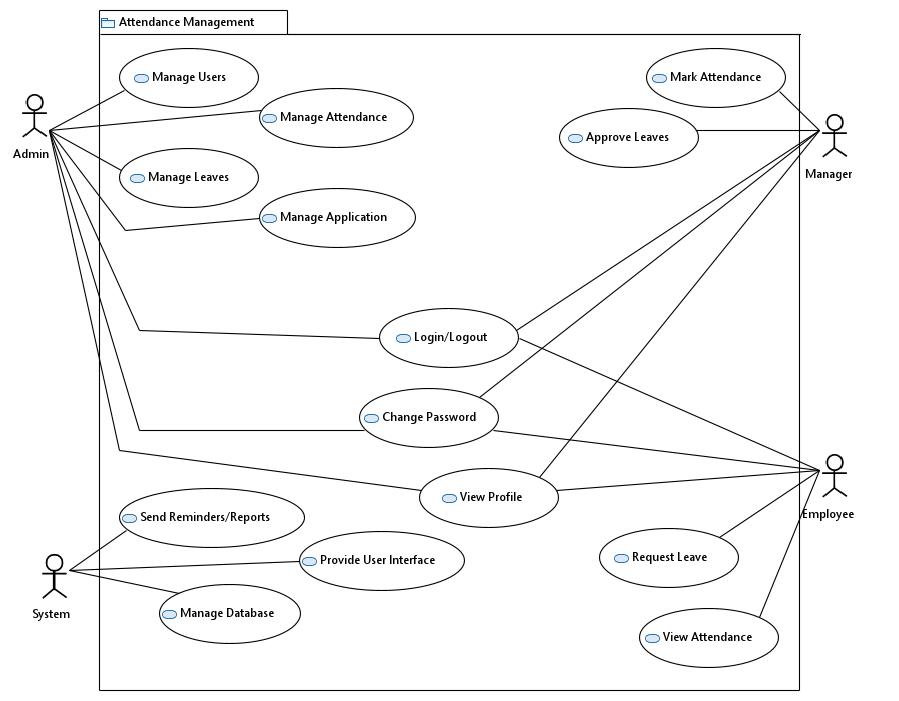
\includegraphics[width=1\textwidth]{Attendance_Management_Use_Case.PNG}\par
\end{center}
\begin{itemize}
    \item \textbf{Actors:}
    \begin{itemize}
        \item Manager
        \item Employee
        \item Administrator
        \item System
    \end{itemize}
    \item \textbf{Manager:}
    \begin{itemize}
        \item Log Attendance: The manager can record a new attendance entry for employees.
        \item Monitor Attendance: The manager can oversee the attendance records of specific employees.
        \item Review Attendance Status: The manager can check the status of each employee’s attendance (present, absent, late).
        \item Edit Attendance: The manager can modify the details of the attendance record.
        \item Remove Attendance Entry: The manager can delete an attendance entry if it is incorrect or no longer needed.
    \end{itemize}
    \newpage
    \item \textbf{Employee:}
    \begin{itemize}
        \item Check Attendance: The employee can review their own attendance records.
        \item Request Leave: The employee can request leave.
    \end{itemize}
    \item \textbf{Administrator:}
    \begin{itemize}
        \item Manage Users (Add/Remove): The administrator can add or remove users from the system.
        \item Assign User Roles: The administrator can designate roles for the users (manager, employee).
        \item Adjust System Settings: The administrator can modify system settings like security protocols, data backups, etc.
    \end{itemize}
    \item \textbf{System:}
    \begin{itemize}
        \item Dispatch Notifications: The system sends alerts regarding attendance logs, updates, etc.
        \item Compile Reports: The system can produce summaries about attendance records, employee punctuality, etc.
    \end{itemize}
\end{itemize}

\subsubsection{Record Employee Attendance}
\begin{center}
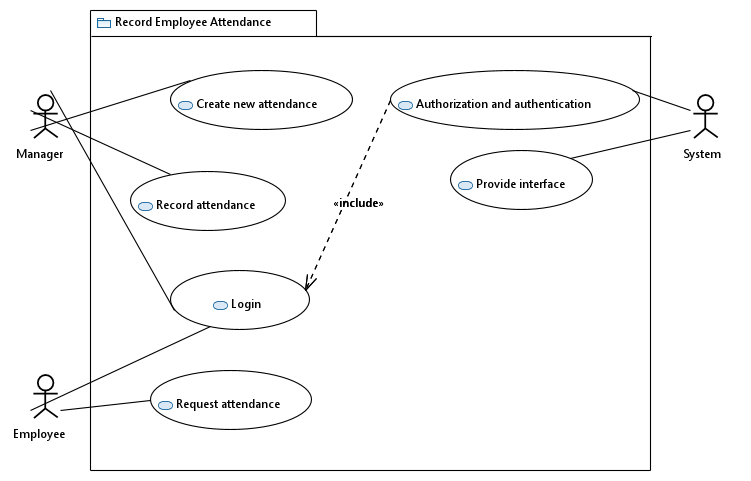
\includegraphics[width=1\textwidth]{Record_Employee_Attendance_Use_Case.PNG}\par
\end{center}
Primary Actor: Employee, Manager\\
Supporting Actor: System\\
Preconditions: The employee is scheduled to work.\\
Postconditions: The employee's attendance record is updated in the system.\\
\newpage
Main Success Scenario:
\begin{enumerate}
    \item The employee arrives at the workplace.
    \item The employee logs into the attendance recording system.
    \item The manager marks the employee's attendance.
    \item The employee begins work.
\end{enumerate}
Extensions:
\begin{itemize}
    \item If the employee encounters technical issues while logging in:
    \begin{enumerate}
        \item The employee notifies the manager.
        \item The manager manually records the employee attendance.
    \end{enumerate}
    \item If the employee forgets to log in:
    \begin{enumerate}
        \item The manager is alerted to the missing entry.
        \item The manager manually records the employee's entry time.
    \end{enumerate}
\end{itemize}

\subsubsection{View Attendance History}
\begin{center}
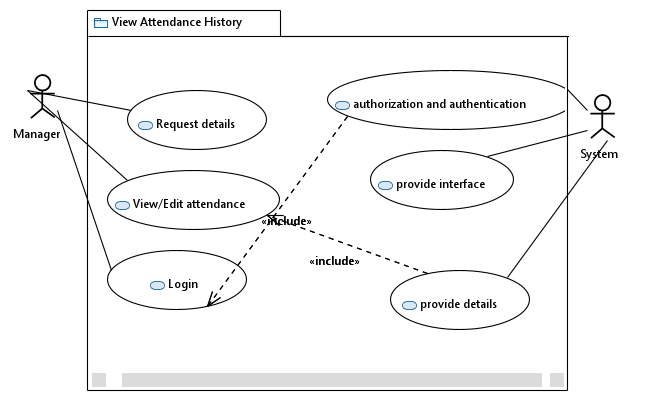
\includegraphics[width=1\textwidth]{View_Attendance_History_Use_Case.PNG}\par
\end{center}
Primary Actor: Manager\\
Supporting Actor: System\\
Preconditions: The manager has valid credentials, and the attendance records are available in the system.\\
Postconditions: Manager views the selected employee's attendance history.\\
\newpage
Main Success Scenario:
\begin{enumerate}
    \item Manager logs in to the attendance management system.
    \item The system validates the credentials and grants access.
    \item Manager selects the "View Attendance History" option.
    \item The system presents a list of employees.
    \item Manager selects a specific employee.
    \item The system retrieves and displays the attendance history of the selected employee.
\end{enumerate}
Extensions:
\begin{itemize}
    \item Invalid Credentials:
    \begin{enumerate}
        \item If the entered credentials are invalid, the system notifies the Manager and prompts them to enter valid credentials.
    \end{enumerate}
    \item No Employees Listed:
    \begin{enumerate}
        \item If there are no employees in the list, the system notifies the Manager that there are no records available.
    \end{enumerate}
\end{itemize}

\subsubsection{Manage Employee Leaves}
\begin{center}
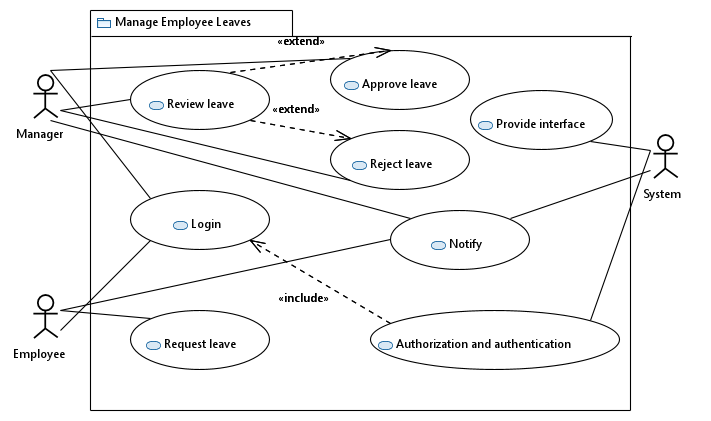
\includegraphics[width=1\textwidth]{Manage_Employee_Leaves_Use_Case.PNG}\par
\end{center}
Primary Actor: Manager, Employee\\
Supporting Actor: System\\
Preconditions: An employee has requested time off.\\
Postconditions: The employee's absence/leave is accurately reflected in the attendance system.\\
\newpage
Main Success Scenario:
\begin{enumerate}
    \item The employee submits a leave request to the manager.
    \item The manager reviews and approves the request.
    \item The attendance database is updated to reflect the approved absence.
\end{enumerate}
Extensions:
\begin{itemize}
    \item If the leave request is denied:
    \begin{enumerate}
        \item The HR manager communicates the decision to the employee.
        \item The employee's attendance record remains unchanged.
    \end{enumerate}
    \item If the employee fails to submit a leave request:
    \begin{enumerate}
        \item The manager follows up with the employee to address the absence.
        \item The absence is recorded as unauthorized in the attendance system.
    \end{enumerate}
\end{itemize}

\newpage
\section{Non-functional Requirements}
\subsection{Performance Requirements}
\begin{itemize}
    \item Response Time: The system is expected to deliver immediate reactions to user inputs to ensure a smooth and efficient user experience.
    \item Concurrent Users: The system is designed to accommodate multiple users simultaneously without noticeable performance issues.
    \item Database Query Performance: Operations involving the retrieval and modification of attendance data should be completed within seconds to promote effective attendance management.
\end{itemize}

\subsection{Safety Requirements}
\begin{itemize}
    \item Data Integrity: Measures must be established to preserve the accuracy and consistency of attendance records, averting any potential data loss or distortion.
    \item User Authentication: A robust authentication system is required to restrict access to authorized users only, safeguarding confidential data.
    \item Backup and Recovery: Consistent backups of the attendance database should be conducted to reduce the risk of data loss, accompanied by a well-defined data recovery strategy in the event of system malfunctions.
\end{itemize}

\subsection{Security Requirements}
\begin{itemize}
    \item Data Encryption: All data exchanges between the user interface and the server are to be encrypted via HTTPS to guarantee data confidentiality and security.
    \item User Authorization: The implementation of role-based access control is essential to limit access to critical features, ensuring that only authorized staff can execute operations such as logging attendance and editing records.
    \item Password Security: Passwords for user accounts must be securely encrypted with hashing algorithms to prevent unauthorized breaches.
    \item Audit Trail: The system is required to keep a comprehensive audit log that records significant actions and transactions for enhanced security and traceability.
\end{itemize}

\subsection{User Documentation}
\begin{itemize}
    \item User Guides: Detailed user guides must be made available to instruct both supervisors and staff on the optimal use of the Employee Attendance Management System.
    \item In-App Support: The application should incorporate a built-in help feature, providing immediate, relevant support and instructional content for users.
    \item Educational Resources: Supplementary educational resources, such as instructional videos or walkthroughs, should be offered to aid in user familiarization and ensure a seamless adaptation to the system.
    \item FAQ Section: An FAQ segment should be present in the documentation to resolve routine inquiries and issues encountered by users.
\end{itemize}

\newpage
\section*{\centering SOFTWARE DESIGN SPECIFICATIONS}

\section{System Architecture}
\subsection{System Level Architecture}
The Employee Attendance Management System is architected as a web-based platform, adhering to the client-server model. This system is structured into several fundamental components:
\begin{itemize}
    \item Frontend (Client-Side):
    \begin{itemize}
        \item Developed with React, the frontend delivers a dynamic and interactive UI for the Employee Attendance Dashboard.
        \item It encompasses modules for managing attendance, user login, and comprehensive dashboard administration.
    \end{itemize}
    \item Backend (Server-Side):
    \begin{itemize}
        \item Utilizing Express, a Node.js web application framework, the backend manages API interactions, user verification, and database communication.
        \item It is tasked with processing user inquiries, validating credentials, database interfacing, and propagating information to the frontend.
    \end{itemize}
    \item Database (DBMS):
    \begin{itemize}
        \item MySQL serves as the database system, organizing and preserving data related to employees and their attendance.
        \item The database maintains tables for employee records, attendance logs, and attendance tracking, ensuring smooth data access and management.
    \end{itemize}
    \item Communication Standards:
    \begin{itemize}
        \item The platform employs HTTP/HTTPS protocols for secure data exchange between the client (web browser) and the server (Express backend).
        \item RESTful APIs are established to streamline the interaction between the frontend and backend, overseeing attendance management, user verification, and other essential operations.
    \end{itemize}
\end{itemize}

\textbf{System Decomposition:}
\begin{itemize}
    \item Client Layer (Frontend):
    \begin{itemize}
        \item Functionalities: Attendance Logging, Hours Monitoring, Access Control, Interface Design.
        \item Roles: Visualize the interface, interact with users, initiate server communication and present data.
    \end{itemize}
    \item Server Layer (Backend):
    \begin{itemize}
        \item Elements: API Services, Authentication Procedures, Database Connectivity.
        \item Roles: Respond to client submissions, authenticate identities, manage database operations, and communicate with the client.
    \end{itemize}
    \newpage
    \item Data Storage Layer (Database):
    \begin{itemize}
        \item Components: Employee Directory, Attendance Records, Attendance Assignments.
        \item Roles: Maintain and organize data on personnel, attendance specifics, and assignment of attendance responsibilities.
    \end{itemize}
\end{itemize}

\textbf{Interaction Protocols:}
\begin{itemize}
    \item Client-Server Dynamics:
    \begin{itemize}
        \item The frontend interfaces with the backend via specified API services, exchanging data in JSON format.
    \end{itemize}
    \item Server-Database Dynamics:
    \begin{itemize}
        \item The backend engages with the MySQL database through SQL operations for data insertion, extraction, modification, and deletion.
    \end{itemize}
\end{itemize}

\textbf{Execution Framework:}
\begin{itemize}
    \item The React framework on the client side is operational within the user’s web browser.
    \item The Express framework on the server side functions on a web server.
    \item The MySQL database system is stationed on a database server, interfaced through XAMPP.
\end{itemize}

\textbf{Global Design Strategies:}
\begin{itemize}
    \item Error Handling:
    \begin{itemize}
        \item A centralized system for error management will be deployed to provide uniform and elucidative error communications to the client when discrepancies occur.
    \end{itemize}
    \item Security Framework:
    \begin{itemize}
        \item Security protocols, including data safeguarding, identity verification, and rights management, will be implemented on both the client and server layers.
    \end{itemize}
\end{itemize}

\subsection{Software Architecture}
The Employee Attendance Management System is structured using a three-tier architecture, which includes the User Interface (UI) Layer, Middle Tier, and Data Access Layer. Below is a detailed description of each layer and the interactions among them:\\
\textbf{Three-Tier Architecture:}
\begin{itemize}
    \item User Interface Layer (Frontend):
    \begin{itemize}
        \item The UI Layer is the visual front that users interact with. It is crafted using React to offer a dynamic and user-friendly Attendance Management Dashboard.
        \item Key functionalities include attendance tracking, leave management, employee authentication, and dashboard administration.
    \end{itemize}
    \newpage
    \item Middle Tier (Backend):
    \begin{itemize}
        \item Serving as the bridge between the UI and the database, the Middle Tier is developed with Express, a Node.js framework.
        \item It manages API requests, executes business logic, and interfaces with the Data Access Layer.
        \item This tier is equipped with API routing, authentication services, and database communication logic.
    \end{itemize}
    \item Data Access Layer (Database Layer):
    \begin{itemize}
        \item Utilizing MySQL as the database system, the Data Access Layer securely stores employee attendance records, personal details, and leave data.
        \item It performs SQL operations for data manipulation, including insertion, retrieval, modification, and deletion.
    \end{itemize}
\end{itemize}
\textbf{Key Interactions:}
\begin{itemize}
    \item From UI Layer to Middle Tier:
    \begin{itemize}
        \item The UI Layer dispatches API calls to the Middle Tier, transmitting data pertinent to attendance management and employee verification.
    \end{itemize}
    \item From Middle Tier to Data Access Layer:
    \begin{itemize}
        \item The Middle Tier executes business rules, interacts with the Data Access Layer, and runs SQL commands on the MySQL database.
    \end{itemize}
    \item From Data Access Layer to Middle Tier:
    \begin{itemize}
        \item The Data Access Layer sends back query outcomes to the Middle Tier, which then processes the information and relays the necessary responses back to the UI Layer.
    \end{itemize}
\end{itemize}

\newpage
\section{Design Strategy}
The design strategy for the Employee Attendance Management System is anchored in principles that ensure flexibility, scalability, and maintainability. The following key considerations have shaped the system’s architecture and high-level organization:
\begin{enumerate}
    \item Future System Extension or Enhancement:
    \begin{itemize}
        \item Strategy: The system’s modular design facilitates straightforward extensions or enhancements.
        \item Reasoning: This modularity allows for seamless integration of new features or updates, enabling the system to evolve with the organization’s needs.
    \end{itemize}
    \item System Reuse:
    \begin{itemize}
        \item Strategy: A three-tier architecture enhances system reuse by delineating the UI, business logic, and data layers.
        \item Reasoning: Independent layer reuse streamlines updates and maintenance, fostering efficient code management.
    \end{itemize}
    \item User Interface Paradigms:
    \begin{itemize}
        \item Strategy: The system leverages React for a responsive and dynamic UI, in line with contemporary UI standards.
        \item Reasoning: An intuitive interface promotes user engagement and adoption, with React enabling a fluid single-page application experience.
    \end{itemize}
    \item Data Management (Storage, Distribution, Persistence):
    \begin{itemize}
        \item Strategy: MySQL is selected for its comprehensive data management capabilities.
        \item Reasoning: MySQL ensures dependable data storage and management, supporting intricate queries and data relationships.
    \end{itemize}
    \item Concurrency and Synchronization:
    \begin{itemize}
        \item Strategy: Asynchronous communication and RESTful APIs are utilized for effective concurrency management.
        \item Reasoning: This approach guarantees a responsive UI and streamlined synchronization, accommodating multiple users simultaneously.
    \end{itemize}
\end{enumerate}
\textbf{Trade-offs:}
\begin{itemize}
    \item The three-tier architecture’s modularity comes with increased deployment and maintenance complexity.
    \item React’s requirement for a modern browser may restrict compatibility for users with outdated browsers.
\end{itemize}

\newpage
\section{Detailed System Design}
\subsection{Database Design}
\subsubsection{Class Diagram}
\begin{center}
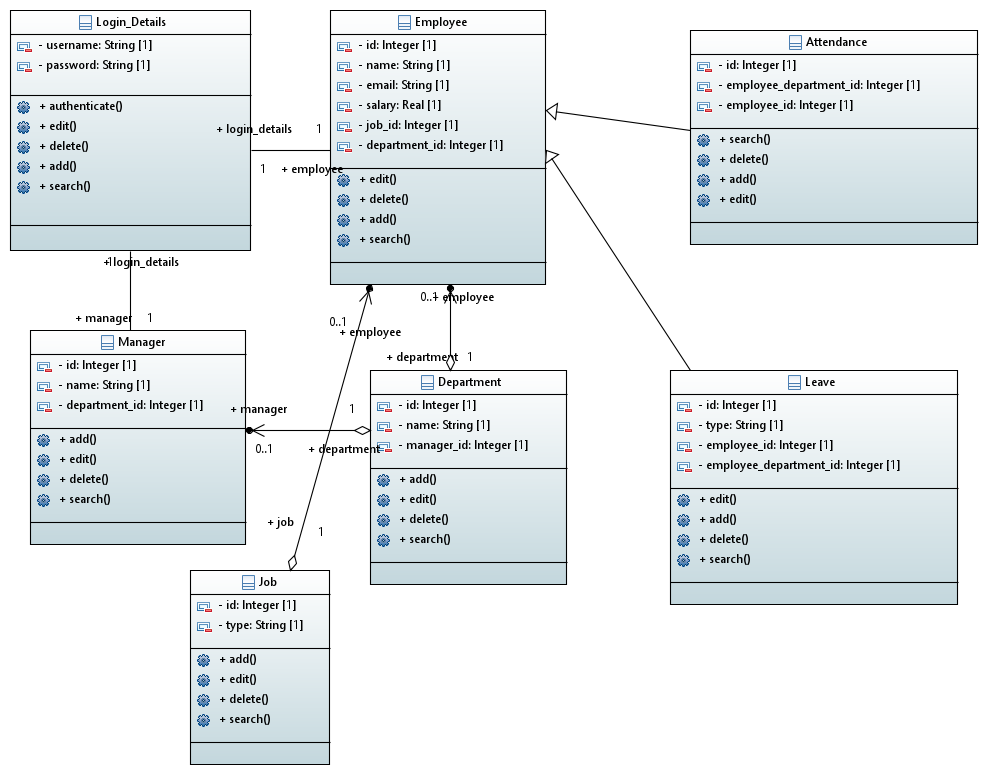
\includegraphics[width=1\textwidth]{Attendance_Management_System_Class_Diagram.PNG}\par
\end{center}
Here’s a detailed description of the classes and their attributes, methods, and interactions:
\begin{enumerate}
    \item Employee: This class represents an employee in the company. It has attributes such as employeeID, name, Salary, departmentID, jobID, and methods like Markarrendance(), updateEmployee(), ApplyLeave(). These methods are used to manage the employee data.
    \item Manager: This class could represent a manager in the company. It is an instance of the Employee class. It has additional methods like manageattendance(), manageleave(), manageDepartment(), addEmployee().
    \item Department: This class represents the various departments within the company. It has attributes like departmentID, departmentName, and methods like addDepartment(), deleteDepartment().
    \item Attendance: This class represents the attendance of employees. It has attributes like id, intime , date, status and methods like addAttendance(), deleteAttendance().
    \item Attendance: This class represents the leaves of employees. It has atributes like leaveid, Startdate, Enddate, reason and methods like addLeave(), deleteLeave().
\end{enumerate}
In the system’s class diagram, the lines symbolize the associations between different classes. These connections illustrate how entities within the system interact with one another. For instance:
\begin{itemize}
    \item An Employee is linked to a Department, indicating that each employee belongs to a specific department. This relationship is depicted by a line connecting the Employee and Department classes.
    \item A Manager has the authority to edit the attendance of an Employee, demonstrating the managerial role in attendance management. This is represented by a line that connects the Manager and Attendance classes to the Employee class.
\end{itemize}
These relationships are crucial for understanding the system’s structure and the flow of information between its components. They ensure that the system accurately reflects the organizational hierarchy and the distribution of responsibilities.
\textbf{Logical Model:}
\begin{center}
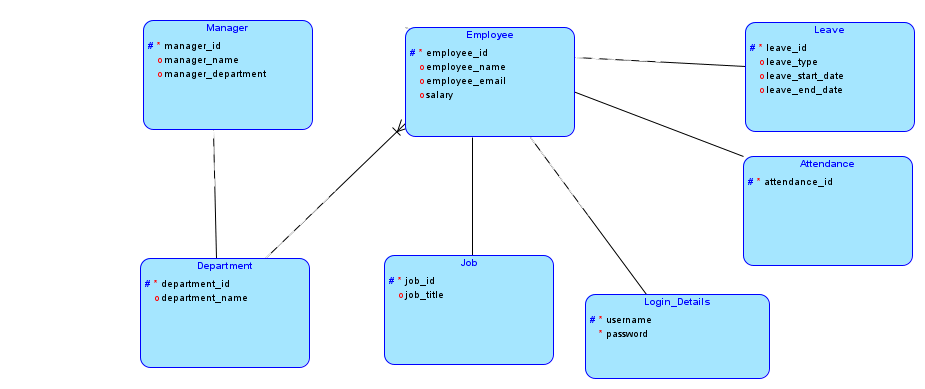
\includegraphics[width=1\textwidth]{Logical.png}\par
\end{center}
\textbf{Relational Model:}
\begin{center}
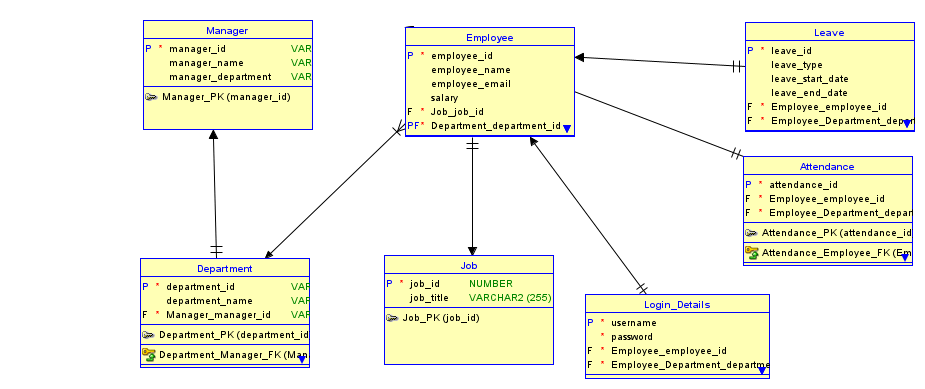
\includegraphics[width=1\textwidth]{Relational.png}\par
\end{center}

\subsubsection{ER Diagram}
\begin{center}
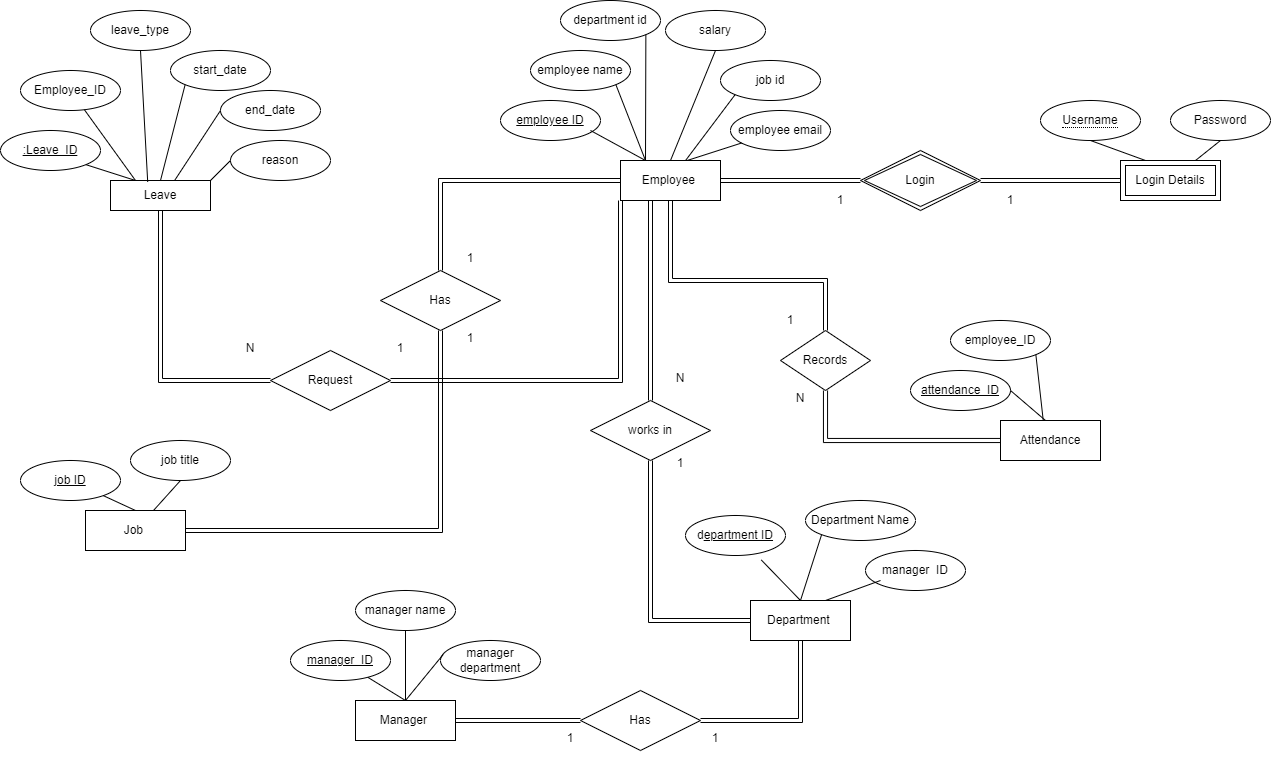
\includegraphics[width=1\textwidth]{Entity_Relation_Diagram.png}\par
\end{center}
Employee Attendance Management System Entities and Relationships
\begin{enumerate}
    \item Employee Entity:
    \begin{itemize}
        \item Represents an individual employee within the system.
        \item Attributes include:
        \begin{itemize}
            \item Name: Full name of the employee.
            \item Job: Designation or role within the company.
            \item Department: Specific department the employee is part of.
            \item Manager: Direct supervisor, potentially linked to another Employee entity.
        \end{itemize}
    \end{itemize}
    \item Attendance Entity:
    \begin{itemize}
        \item Denotes the Attendnaces of all the employees.
        \item Attributes encompass:
        \begin{itemize}
            \item id: Refer to employee id from employees.
            \item intime: Time of attendance.
            \item Date: Date of a particular attendance.
            \item Status: refers to the status of employee present absent or leave (e.g. 'A', 'P', 'L').
        \end{itemize}
    \end{itemize}
    \item Relationships and Multiplicity:
    \begin{itemize}
        \item The connections between entities are depicted through lines in the class diagram.
        \item Multiplicity, or the cardinality of a relationship, is denoted by numerical values or symbols adjacent to the entities. For instance:
        \begin{itemize}
            \item A “1” near the Manager entity and an “N” near the Employee entity signifies that a single manager may be linked to multiple employees.
            \item A “1” near both entities indicates one-to-one relationships.
        \end{itemize}
    \end{itemize}
\end{enumerate}

\subsubsection{Data Dictionary}
\textbf{User Information:\\\\}
\begin{tabular}{|c|c|c|c|c|c|c|}
    \hline
    \textbf{Column} & \textbf{Description} & \textbf{Type} & \textbf{Length} & \textbf{Nullable} & \textbf{Default} & \textbf{Key} \\
    \hline
    id & Unique identifier for each user & Integer & & No & Auto & PK \\
    \hline
    name & Username chosen by the user & Text & 50 & No & & \\
    \hline
    email & Email address of the user & Text & 100 & No & & \\
    \hline
    password & Hashed password authentication & Text & & No & & \\
    \hline
\end{tabular}
\\\\
\textbf{Attendance Information:\\\\}
\begin{tabular}{|c|c|c|c|c|c|c|}
    \hline
    \textbf{Column} & \textbf{Description} & \textbf{Type} & \textbf{Length} & \textbf{Nullable} & \textbf{Default} & \textbf{Key} \\
    \hline
    employee\_id & Foreign key referencing Employees & Integer & & No & & FK \\
    \hline
    In\_time & Time of marking the attendance & Time & 100 & No & Current & \\
    \hline
    Date & Date of attendance & Date & & Yes & Current & \\
    \hline
    status & Status of presence & Char & & No & - & \\
    \hline
\end{tabular}
\\\\
\textbf{Manager Information:\\\\}
\begin{tabular}{|c|c|c|c|c|c|c|}
    \hline
    \textbf{Column} & \textbf{Description} & \textbf{Type} & \textbf{Length} & \textbf{Nullable} & \textbf{Default} & \textbf{Key} \\
    \hline
    manager\_id & Unique identifier for each manager & Integer & & No & Auto & PK \\
    \hline
    name & Name of the manager & Text & & No & & \\
    \hline
\end{tabular}

\newpage
\section{Application Design}
\subsection{Sequence Diagram}
The sequence diagram illustrates the dynamic interactions among various components of the system, specifically focusing on the user, web page, database, employee dashboard, and manager dashboard. It delineates the distinct capabilities allocated to managers and employees. Detailed explanation:
\begin{enumerate}
    \item User Interaction with Web Page:
    \begin{itemize}
        \item Initially, the user accesses the web page and inputs their credentials, typically through a login procedure involving a username and password.
    \end{itemize}
    \item Redirection to Dashboards:
    \begin{itemize}
        \item Post-authentication, the system identifies the user’s role. Managers are directed to the manager dashboard, while other employees see the employee dashboard, indicating tailored interfaces for different user types.
    \end{itemize}
    \item Employee Dashboard Functions:
    \begin{itemize}
        \item Within the employee dashboard, users can:
        \begin{itemize}
            \item View Attendance: Check their attendance records and history.
            \item Record Attendance: Mark their arrival and departure times, which are then logged in the database.
            \item Request Leave: Submit leave applications for approval, which are also tracked in the database.
        \end{itemize}
    \end{itemize}
    \item Manager Dashboard Functions:
    \begin{itemize}
        \item The manager dashboard allows managers to:
        \begin{itemize}
            \item View Attendance Records: Oversee the attendance details of all employees.
            \item Approve Leave: Review and approve leave requests from employees, with updates reflected in the database.
            \item Manage Schedules: Adjust employee schedules and shifts, ensuring accurate attendance tracking.
        \end{itemize}
    \end{itemize}
    \item Database Interactions:
    \begin{itemize}
        \item The database plays a pivotal role in retrieving employee details and logging new attendance. It is updated in real-time as records are added or removed.
    \end{itemize}
\end{enumerate}
\subsubsection{Attendance Management Sequence}
\begin{center}
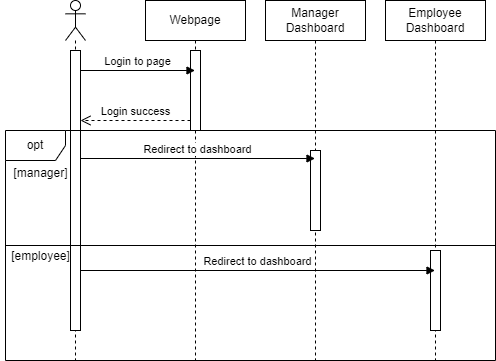
\includegraphics[width=1\textwidth]{Attendance Management Sequence.png}\par
\end{center}
\subsubsection{Login Sequence}
\begin{center}
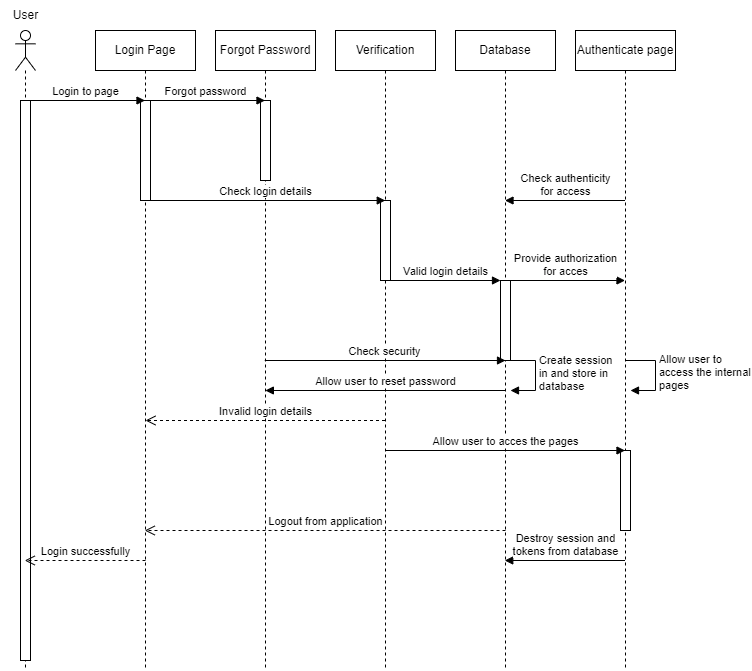
\includegraphics[width=1\textwidth]{Login Sequence.png}\par
\end{center}
\subsubsection{Manager Sequence}
\begin{center}
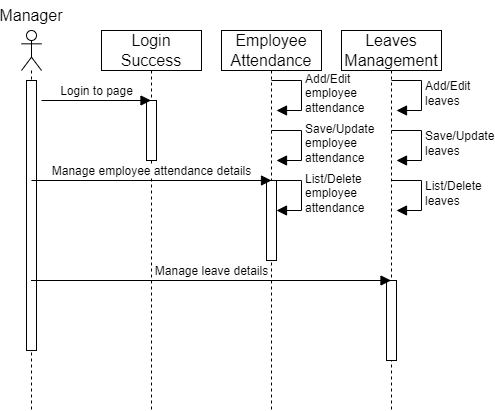
\includegraphics[width=1\textwidth]{Manager Sequence.png}\par
\end{center}
\subsubsection{Employee Sequence}
\begin{center}
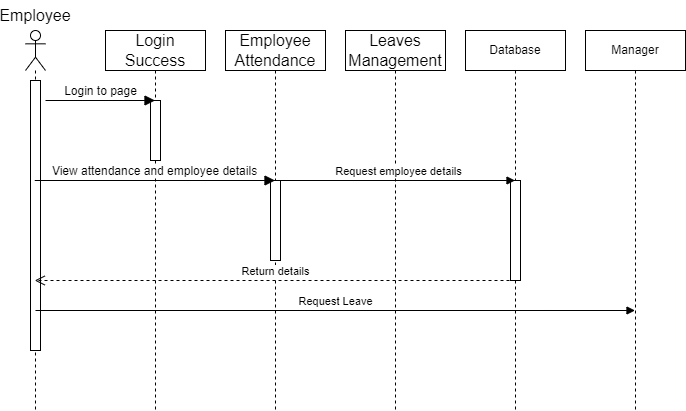
\includegraphics[width=1\textwidth]{Employee Sequence.png}\par
\end{center}

\subsection{State Chart Diagram}
\begin{center}
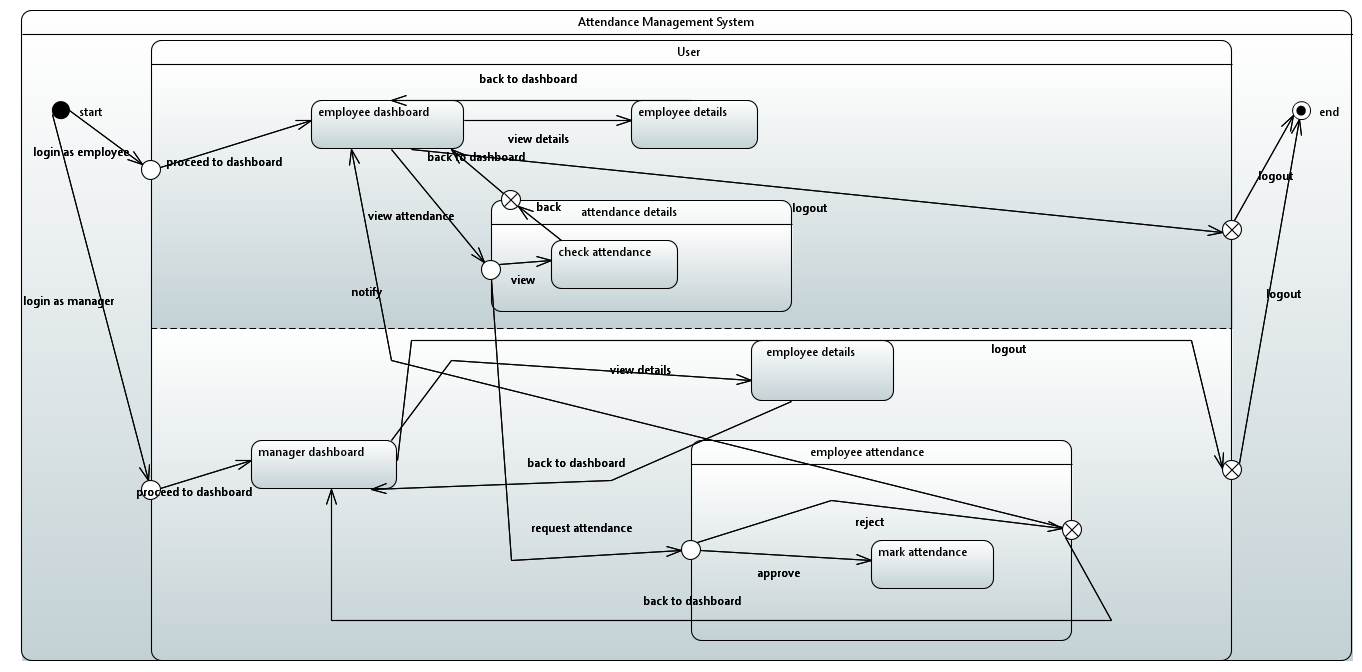
\includegraphics[width=1\textwidth]{Attendance_Management_System_State_Chart.PNG}\par
\end{center}
\begin{enumerate}
    \item Employee States: The diagram’s upper section outlines the potential states for an employee.
    \begin{itemize}
        \item EmployeeDashboard: The default state where employees can view their attendance records.
        \item RecordAttendance: In this state, employees log their attendance.
        \item OnLeave: This state indicates that the employee is on approved leave.
        \item Present: This state signifies that the employee is marked present for the day.
        \item Absent: This state indicates an unrecorded or missed attendance.
        \item LoggedOut: This state occurs when the employee logs out of the system.
    \end{itemize}
    \item Manager States: The lower section of the diagram depicts the states a manager can experience.
    \begin{itemize}
        \item ManagerDashboard: The initial state where managers can oversee attendance and leave requests.
        \item ApproveLeave: In this state, managers approve or reject leave applications.
        \item ReviewAttendance: Managers enter this state to review and manage attendance discrepancies.
        \item CompletedReview: This state signifies the completion of attendance review.
        \item TerminatedReview: This state occurs if a review process is canceled or terminated.
        \item LoggedOut: This state represents the manager logging out of the system.
    \end{itemize}
    \item Transitions: Arrows illustrate the state transitions triggered by specific actions. For instance, an employee moves from the “EmployeeDashboard” to “RecordAttendance” when they log their arrival. Similarly, a manager transitions from “ManagerDashboard” to “ApproveLeave” upon initiating the leave approval process.
\end{enumerate}

\subsection{Activity Diagram}
\textbf{Employee Activity:}
\begin{enumerate}
    \item Employee Activity: The process begins with the employee logging into the system.
    \item Web Page: Upon successful login, the employee is navigated to the dashboard where they can record attendance, view attendance history, and view personal details.
    \item Database: This stage involves the verification of the employee’s credentials during login. If the credentials are validated, access to the dashboard is granted. Otherwise, the employee is prompted to retry the login.
    \item Flow of Activities: The arrows in the diagram indicate the sequence of actions. For instance, post-login, the employee may opt to mark attendance, review their attendance records, or request leave.
    \item Decision Points: Diamond shapes in the diagram depict decision-making junctures. For example, following a login attempt, the system assesses the authenticity of the credentials. If they are accurate, the employee proceeds to the dashboard; if not, a login retry is required.
\end{enumerate}
\textbf{Manager Activity:}
\begin{enumerate}
    \item Manager Dashboard: The process initiates with the manager logging into the system.
    \item Web Page: Following a successful login, the manager is taken to the dashboard where they can add, view, and remove employee records.
    \item Database: This stage pertains to the authentication of the manager’s credentials during login. Correct credentials lead to dashboard access, while incorrect ones result in redirection to the login page.
    \item Flow of Activities: The arrows signify the sequence of actions. For instance, after logging in, the manager may decide to register new employees, inspect attendance records, or manage employee details.
    \item Decision Points: Diamond shapes indicate critical decision points. For example, post-login attempt, the system evaluates the credentials’ validity. If they are verified, the manager accesses the dashboard; if not, they are prompted to log in again.
\end{enumerate}
\subsubsection{Attendance Management System Activity Diagram}
\begin{center}
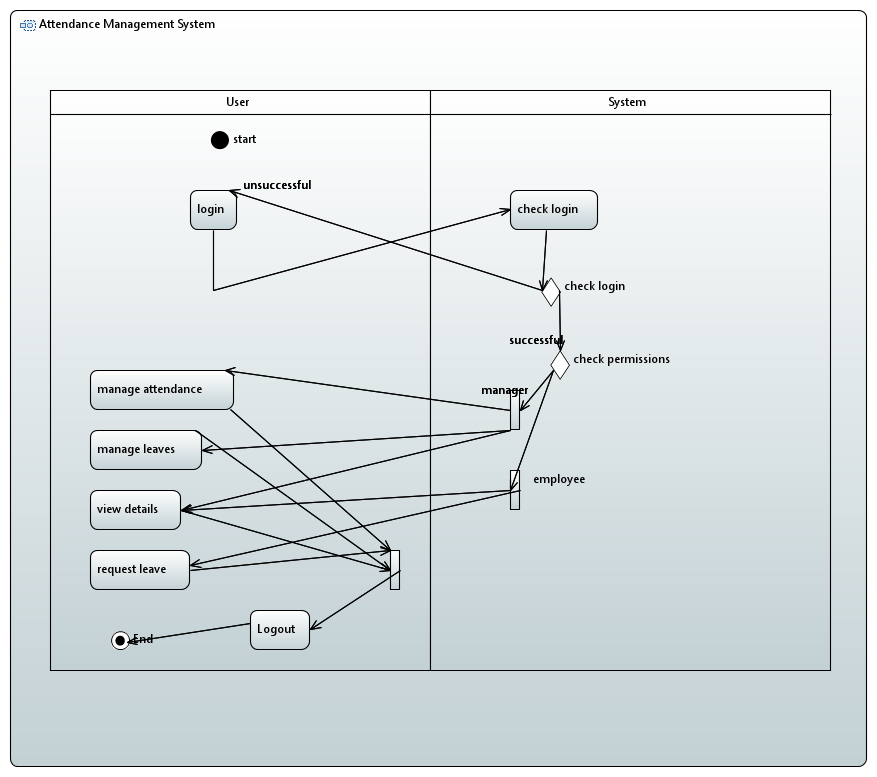
\includegraphics[width=1\textwidth]{Attendance_Management_System_Activity_Diagram.PNG}\par
\end{center}
\subsubsection{Employee Attendance Activity Diagram}
\begin{center}
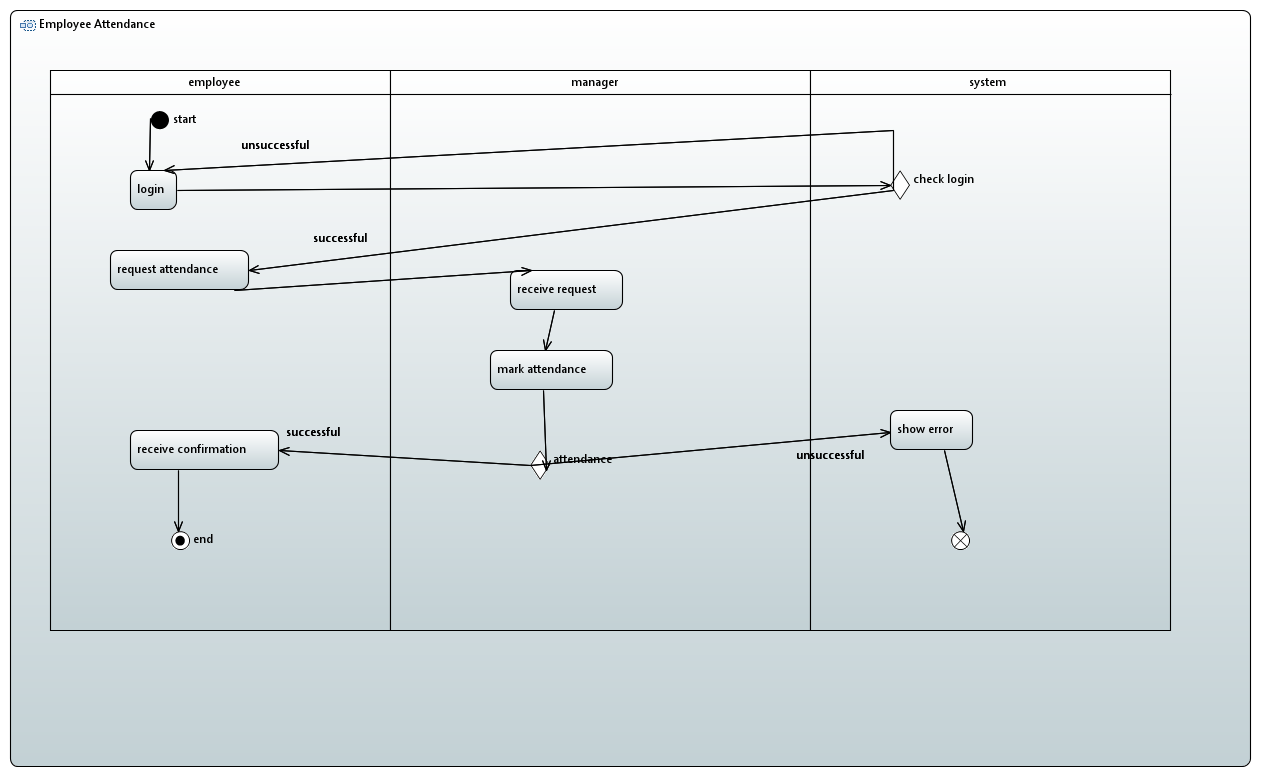
\includegraphics[width=1\textwidth]{Employee_Attendance_Activity_Diagram.PNG}\par
\end{center}
\subsubsection{Employee Registration Activity Diagram}
\begin{center}
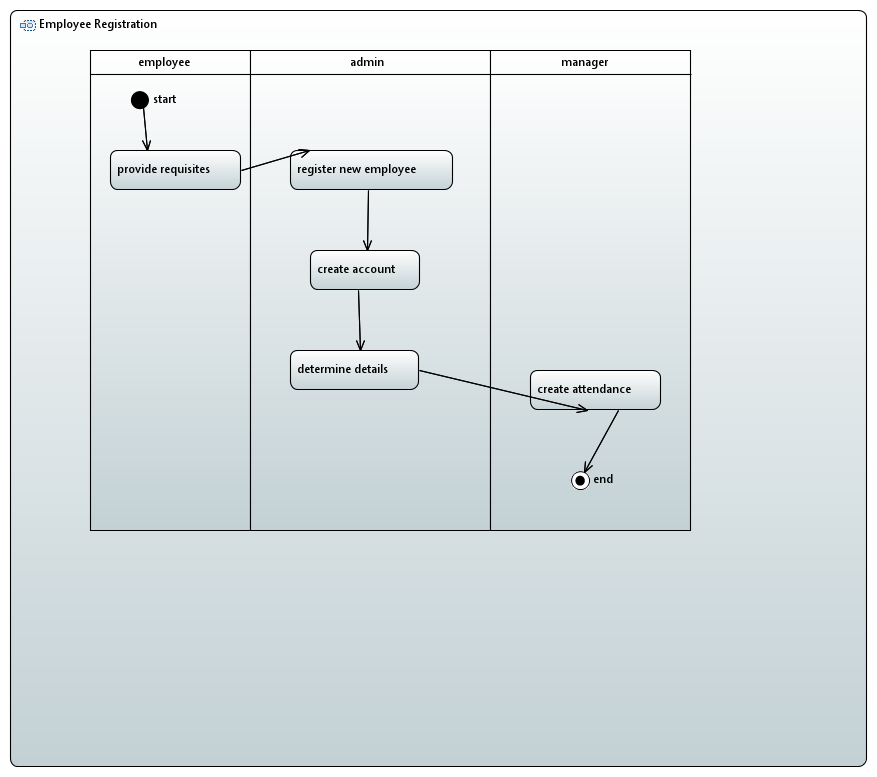
\includegraphics[width=1\textwidth]{Employee_Registration_Activity_Diagram.PNG}\par
\end{center}
\subsubsection{Set Permissions Activity Diagram}
\begin{center}
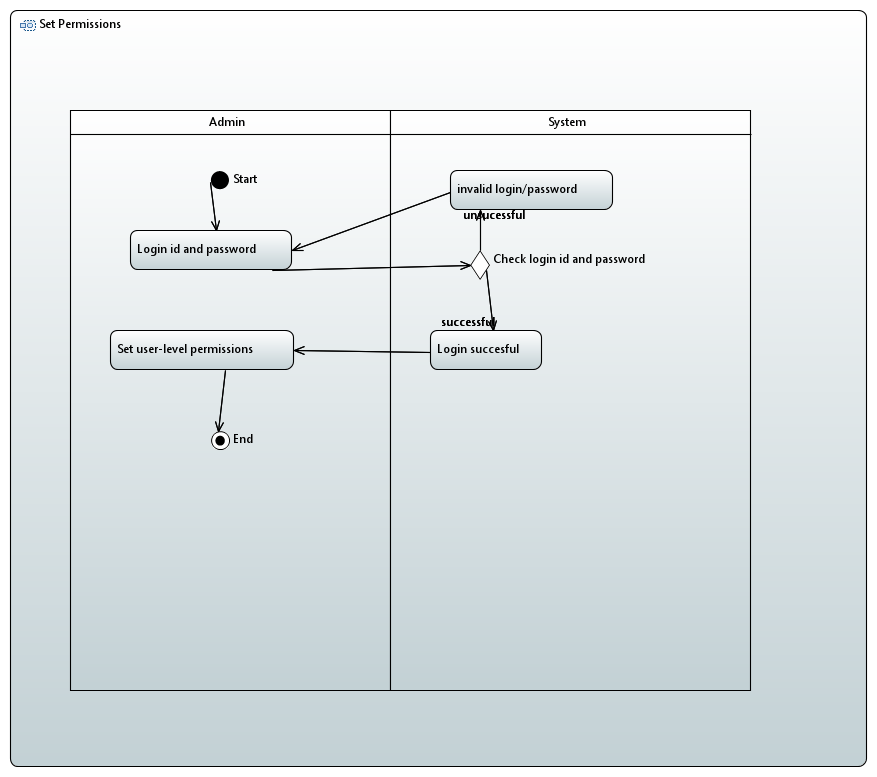
\includegraphics[width=1\textwidth]{Set_Permissions_Activity_Diagram.PNG}\par
\end{center}

\subsection{Component Diagram}
\begin{center}
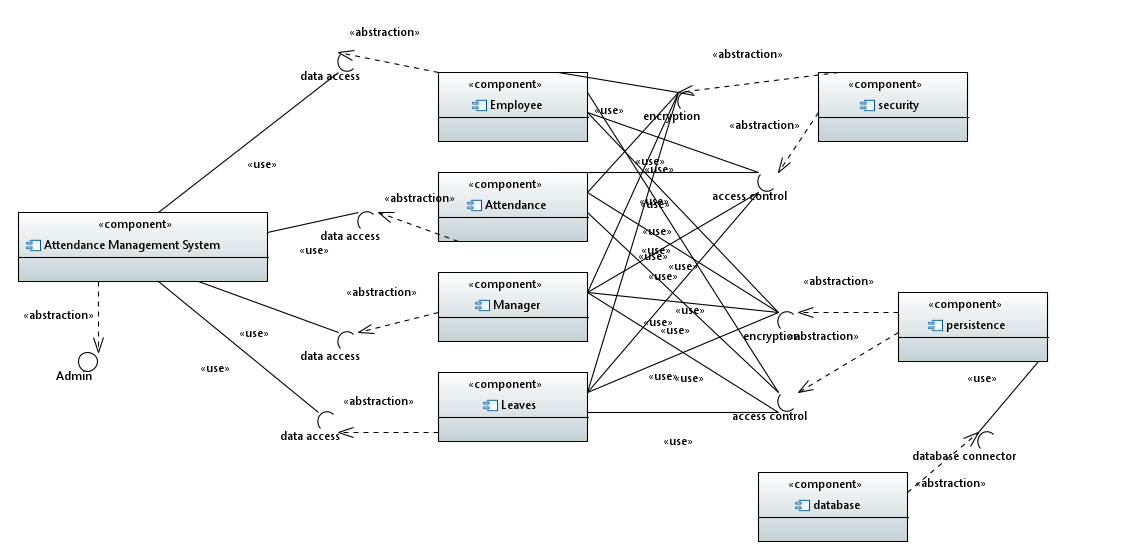
\includegraphics[width=1\textwidth]{Attendance_Management_System_Component_Diagram.PNG}\par
\end{center}
Breakdown of Component Diagram:
\begin{enumerate}
    \item System Components: The diagram outlines the core system components.
    \begin{itemize}
        \item User Interface: The primary interface for user interaction with the attendance management application.
        \item View Controller: This component manages the display content on the user interface.
        \item Model: Represents the attendance data and the business logic for data access and updates.
        \item Database: The storage system for all attendance-related data.
    \end{itemize}
    \item User Interface Components: The diagram details the user interface components.
    \begin{itemize}
        \item Login: Manages the authentication process for users.
        \item Attendance Dashboard: The central hub for users to manage attendance records.
    \end{itemize}
    \item Relationships: The connecting lines in the diagram depict the inter-component relationships. The arrow direction shows dependency, such as the User Interface relying on the View Controller for display logic.
\end{enumerate}

\subsection{Deployment Diagram}
\begin{center}
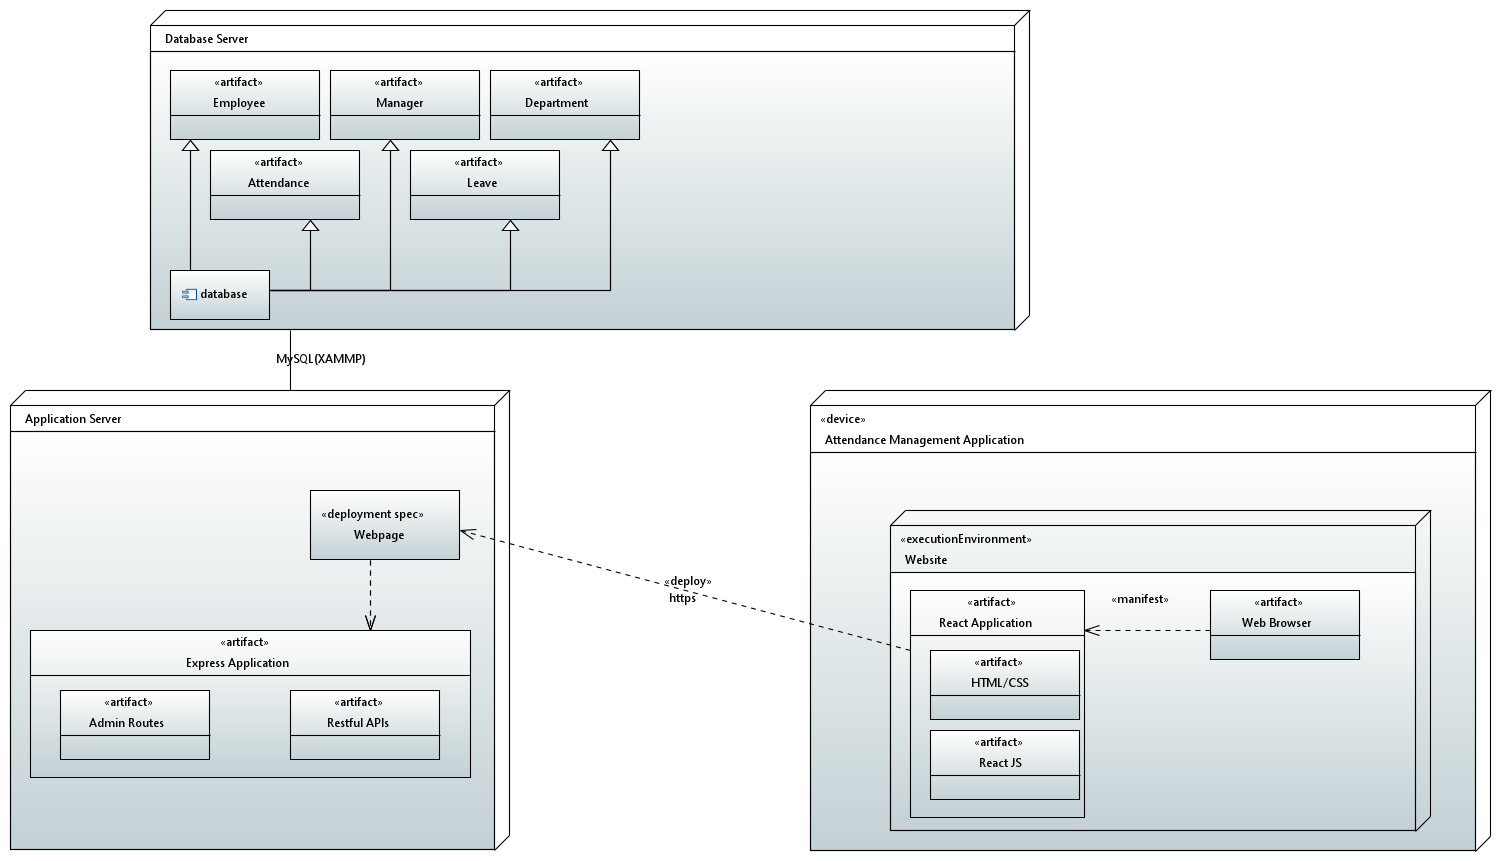
\includegraphics[width=1\textwidth]{Attendance_Management_System_Deployment_Diagram.PNG}\par
\end{center}
Breakdown of the Deployment Diagram:
\begin{enumerate}
    \item Client Device: Represents the user’s device, such as a web browser or mobile app, where the application’s user interface is accessed.
    \item Web Server: Hosts the Express and Node.js application.
    \begin{itemize}
        \item Attendance Module: Manages the recording, viewing, and updating of attendance records.
        \item Leave Management Module: Handles leave requests and approvals.
    \end{itemize}
    \item Database Server: The MySQL database server.
    \begin{itemize}
        \item Employee Table: Stores data related to employee profiles and attendance.
        \item Leave Table: Maintains records of leave applications and statuses.
    \end{itemize}
\end{enumerate}

\newpage
\section{References \& Citations}
% Your references content here
\begin{itemize}
    \item MySQL Documentation:\\
    \href{https://dev.mysql.com/doc/}{$Source: MySQL Official Documentation$}
    \item Express Documentation:\\
    \href{http://expressjs.com/}{Source: Express Official Documentation}
    \item React Documentation:\\
    \href{https://legacy.reactjs.org/}{Source: React Official Documentation:}
    \item Node.js Documentation:\\
    \href{https://nodejs.org/en/docs}{Source: Node.js Official Documentation}
    \item HTML/CSS Documentation:\\
    \href{https://developer.mozilla.org/en-US/}{Source: MDN Web Docs}
    \item JavaScript Documentation:\\
    \href{https://developer.mozilla.org/en-US/docs/Web/javascript}{Source: MDN Web Docs JavaScript}
\end{itemize}

\newpage
\section{Appendices}
\subsection{Project Timeline}
\subsubsection{Week 1}
Tasks:
\begin{itemize}
    \item Research and Planning:
    \begin{itemize}
        \item Define detailed project requirements for attendance tracking.
        \item Finalize the user stories and features for attendance management.
    \end{itemize}
    \item Environment Setup:
    \begin{itemize}
        \item Install and configure development tools (Node.js, MySQL).
        \item Set up the project structure for the attendance system.
    \end{itemize}
\end{itemize}
Updates:
\begin{itemize}
    \item Research completed, and project requirements for attendance management documented.
    \item Development environment for attendance system configured successfully.
\end{itemize}

\subsubsection{Week 2}
Tasks:
\begin{itemize}
    \item Database Design:
    \begin{itemize}
        \item Create the Entity-Relationship Diagram (ERD) for attendance data.
        \item Set up the MySQL database with tables for employee attendance records.
    \end{itemize}
    \item Backend Development:
    \begin{itemize}
        \item Develop the Express.js backend server for attendance operations.
        \item Implement database operations for attendance CRUD functionality.
    \end{itemize}
\end{itemize}
Updates:
\begin{itemize}
    \item ERD for attendance management completed and database structure defined.
    \item Basic backend functionality for attendance operations implemented.
\end{itemize}

\subsubsection{Week 3}
Tasks:
\begin{itemize}
    \item Frontend Development:
    \begin{itemize}
        \item Set up the React.js frontend application for attendance interface.
        \item Create components for recording, viewing, updating, and deleting attendance records.
    \end{itemize}
    \item Integration:
    \begin{itemize}
        \item Connect the frontend and backend to ensure seamless data flow for attendance management.
    \end{itemize}
\end{itemize}
Updates:
\begin{itemize}
    \item Basic frontend structure for attendance management in place.
    \item Initial integration between frontend and backend for attendance system achieved.
\end{itemize}

\subsubsection{Week 4}
Tasks:
\begin{itemize}
    \item User Interface Refinement:
    \begin{itemize}
        \item Improve the UI for a better user experience in attendance tracking.
        \item Implement features for attendance reporting, leave requests, and employee scheduling.
    \end{itemize}
    \item Testing:
    \begin{itemize}
        \item Begin testing phases (unit testing and integration testing) for attendance system.
    \end{itemize}
\end{itemize}
Updates:
\begin{itemize}
    \item UI enhancements for attendance management completed.
    \item Initial testing phase for attendance system started.
\end{itemize}

\subsubsection{Week 5}
Tasks:
\begin{itemize}
    \item Testing and Debugging:
    \begin{itemize}
        \item Conduct thorough testing of the entire attendance application.
        \item Address and resolve any bugs or issues identified in the attendance system.
    \end{itemize}
    \item Documentation:
    \begin{itemize}
        \item Create user manuals and documentation for the attendance management system.
    \end{itemize}
\end{itemize}
Updates:
\begin{itemize}
    \item Testing phase for attendance system ongoing, with identified bugs being addressed.
    \item Initial draft of user manuals for attendance system completed.
\end{itemize}

\end{document}